\documentclass[11pt,a4j,openany,fleqn]{jbook}

\usepackage{times}
\usepackage{multirow}
\usepackage{amsmath}
\usepackage{color}
\usepackage{here}
\usepackage{graphicx}
\usepackage{array}
\usepackage{booktabs}
\usepackage{threeparttable}
\usepackage{url}
\usepackage{listings,makeidx}
\usepackage{fancyhdr}
\usepackage{fancybox}
\usepackage{ascmac}
\usepackage{color}
\usepackage[titles]{tocloft}

\graphicspath{{./fig/}}

\setcounter{secnumdepth}{3}
\setcounter{tocdepth}{3}

\makeatletter
\def\thanks#1{%
  \footnotemark
  \edef\@tempa{\noexpand\noexpand\noexpand\footnotetext[\the\c@footnote]}%
  \toks@\expandafter{\@thanks}%
  \toks\tw@{{#1}}
  \xdef\@thanks{\the\toks@\@tempa\the\toks\tw@}} 
\def\ps@mybothstyle{\let\ps@jpl@in\ps@plain
\def\@evenhead{\leftmark\hfil}
\def\@evenfoot{\hfil\hfil}
\def\@oddhead{\hfil\thepage\rightmark}
\def\@oddfoot{\hfil\hfil}
\let\@mkboth\markboth
\def\sectionmark##1{\markboth{\ifnum \c@secnumdepth >\z@ \thesection.\hskip1zw\fi##1}{}}
\def\subsectionmark##1{\markright{\ifnum \c@secnumdepth >\@ne \thesubsection.\hskip1zw\fi##1}}}
\def\@listI{
  \parsep 3pt
  \topsep 10pt
  \itemsep 0pt
  \parskip 0pt
  \leftskip -10pt
  \leftmargin\leftmargini \addtolength{\leftmargin}{\leftskip}
}
\renewcommand{\thefootnote}{\,注\arabic{footnote}\,}
\renewcommand{\tableofcontents}{%
  \if@twocolumn\@restonecoltrue\onecolumn
  \else\@restonecolfalse\fi
  \section*{\contentsname
    \@mkboth{\contentsname}{\contentsname}%
  }\@starttoc{toc}%
  \if@restonecol\twocolumn\fi
}
\renewenvironment{thebibliography}[1]
{\section*{\bibname\@mkboth{\bibname}{\bibname}}%
   \list{\@biblabel{\@arabic\c@enumiv}}%
        {\settowidth\labelwidth{\@biblabel{#1}}%
         \leftmargin\labelwidth
         \advance\leftmargin\labelsep
         \@openbib@code
         \usecounter{enumiv}%
         \let\p@enumiv\@empty
         \renewcommand\theenumiv{\@arabic\c@enumiv}}%
   \sloppy
   \clubpenalty4000
   \@clubpenalty\clubpenalty
   \widowpenalty4000%
   \sfcode`\.\@m}
  {\def\@noitemerr
    {\@latex@warning{Empty `thebibliography' environment}}%
   \endlist}

\renewcommand{\maketitle}{\begin{titlepage}%
  \let\footnotesize\small
  \let\footnoterule\relax
  \let\footnote\thanks
  \null\vfil
  \vskip 60\p@
  \begin{center}%
    {\LARGE \@title \par}%
    \vskip 3em%
    {\Large
     \lineskip .75em%
      \begin{tabular}[t]{c}%
        \@author
      \end{tabular}\par}%
      \vskip 0.5em%
    {\large \@date \par}%       % Set date in \large size.
    \vskip 2em%
    \titleadd
  \end{center}\par
  \vskip 5em%
  {\copyrighttext\par}%
  \@thanks\vfil\null
  \end{titlepage}%
  \setcounter{footnote}{0}%
  \global\let\thanks\relax
  \global\let\maketitle\relax
  \global\let\p@thanks\relax
  \global\let\@thanks\@empty
  \global\let\@author\@empty
  \global\let\@date\@empty
  \global\let\@title\@empty
  \global\let\title\relax
  \global\let\author\relax
  \global\let\date\relax
  \global\let\and\relax
  }%
%\renewcommand{\thefigure}{%
%\thesection\arabic{figure}}
%\@addtoreset{figure}{section}
%\renewcommand{\thetable}{%
%\thesection\arabic{table}}
%\@addtoreset{table}{section}
\makeatother

\newcommand{\percent}{\%}
\renewcommand{\lstlistingname}{Spur_fail1.c}
\lstset{%
 language={bash},
 backgroundcolor={\color[gray]{0.90}},%
 basicstyle={\small\ttfamily},%
 identifierstyle={\small\ttfamily},%
 commentstyle={\small\slshape},%
 keywordstyle={\small\ttfamily},%
 ndkeywordstyle={\small\ttfamily},%
 stringstyle={\small\ttfamily},
 frame={tb},
 breaklines=true,
 breakindent=2em,
 numbers=left,%
 xrightmargin=0.5zw,%
 xleftmargin=1.5zw,%
 numberstyle={\scriptsize},%
 stepnumber=1,
 numbersep=1zw,%
 lineskip=-0.5ex,%
 tabsize=4
}
\DeclareFontShape{JY1}{mc}{m}{sl}{<5> <6> <7> <8> <9> <10> sgen*min
    <10.95><12><14.4><17.28><20.74><24.88> min10
    <-> min10}{}
\DeclareFontShape{JT1}{mc}{m}{sl}{<5> <6> <7> <8> <9> <10> sgen*tmin
    <10.95><12><14.4><17.28><20.74><24.88> tmin10
    <-> tmin10}{}

\renewcommand{\topfraction}{1.00}
\renewcommand{\bottomfraction}{1.00}
\renewcommand{\textfraction}{0.00}
\renewcommand{\floatpagefraction}{1.00}
\renewcommand{\dbltopfraction}{1.00}
\renewcommand{\dblfloatpagefraction}{1.00}

\renewcommand{\contentsname}{\Large 目次}
\renewcommand{\bibname}{\Large 参考文献}

\setlength\floatsep{6pt}
\setlength\textfloatsep{6pt}
\setlength\intextsep{6pt}
\setlength\abovecaptionskip{0pt}

\setlength{\topmargin}{0truemm}
\setlength{\textheight}{241truemm}
\setlength{\headheight}{6truemm}
\setlength{\headsep}{8truemm}
\setlength{\oddsidemargin}{0truemm}
\setlength{\evensidemargin}{0truemm}
\setlength{\textwidth}{160truemm}
\setlength{\columnsep}{8truemm}
\setlength{\skip\footins}{4truemm}

\setlength{\baselineskip}{5truemm}
\setlength{\parskip}{1truemm}

\hyphenpenalty=10000\relax
\sloppy

\newcommand{\rev}{rev.6 - December 6, 2016}
\newcommand{\authorname}{渡辺 敦志 (WATANABE Atsushi)}
\newcommand{\papertitle}{二軸ブラシレスモータドライバ TF-2MD3-R6 User's Manual}


\usepackage{atbegshi}
\AtBeginShipoutFirst{\special{pdf:tounicode 90ms-RKSJ-UCS2}}
\usepackage[setpagesize=false,dvipdfm,
		bookmarks=true,
		bookmarksnumbered=true,
		bookmarksopen=true,
		pdftitle={\papertitle},
		pdfauthor={\authorname},
		colorlinks=false,
		pdfborderstyle={},
%		draft
	]{hyperref}
\setlength{\skip\footins}{12pt}

\urlstyle{sf}

% タイトル
\title{\papertitle}
\author{
\authorname
\thanks{atsushi.w[at]ieee.org}
}
\date{\rev}
\newcommand{\titleadd}{{\includegraphics[width=130mm]{driver_board_r6.eps}}}
\newcommand{\copyrighttext}{\small 
この文章はクリエイティブ・コモンズ・ライセンス 表示 - 継承 3.0 非移植 の下に提供されています。このライセンスのコピーを見るためには、{\scriptsize \url{http://creativecommons.org/licenses/by-sa/3.0/}} をご覧になるか、以下へお手紙をお送り下さい: Creative Commons, 444 Castro Street, Suite 900, Mountain View, California, 94041, USA. \\%[]
\hfill{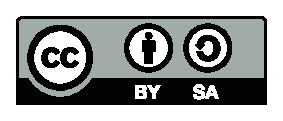
\includegraphics[width=21mm]{by-sa.eps}}
}

\renewcommand{\thesection}{\arabic{section}.}
\renewcommand{\thesubsection}{\arabic{section}.\arabic{subsection}}
\renewcommand{\thesubsubsection}{\arabic{section}.\arabic{subsection}.\arabic{subsubsection}}
\newlength{\boxwidth}
\newlength{\itemwidth}



\newcommand \warnbox [2]{
	\bigskip
	\vbox{
		\setlength{\boxwidth}{\textwidth}
		\addtolength{\boxwidth}{1.05pt}
		{
			\bfseries\large
			\hbox{\rule{\boxwidth}{1.5em}\vspace{-1.8em}}
			\hbox{\hspace{1em}\color{white}{#1}\vspace{-1em}}
		}
		\vspace{-4pt}
		\addtolength{\boxwidth}{-5em}
		\begin{itembox}[l]{\hspace{\boxwidth}}
			\null
			\bigskip
			{#2}
			\null
		\end{itembox}
	}
	\bigskip
}
\newcommand \iconitem [2]{
	\begin{minipage}[m]{13mm}
		\centering\includegraphics[width=12mm]{#1}
	\end{minipage}
	\setlength{\itemwidth}{\textwidth}
	\addtolength{\itemwidth}{-13mm}
	\addtolength{\itemwidth}{-8.5pt}
	\begin{minipage}[m]{\itemwidth}
		\begin{itemize}
			#2
		\end{itemize}
	\end{minipage}
}
\newcommand \itemseprule {
	\vspace{5pt}
	\hrule
	\vspace{5pt}
}

\newcommand \urllink [1]{
	\vspace{5pt}
	\ovalbox{
		\small\url{#1}
	}
	\vspace{5pt}
}



\begin{document}
\frontmatter
\maketitle

\newpage
\thispagestyle{fancy}
\fancyhead{}
\fancyhead[LO,LE]{\papertitle \;\;(\rev)}
\fancyhead[RO,RE]{改訂履歴}
\cfoot{}

\vspace{10mm}\hbox{}
\begin{center}
{\bf\large 改訂履歴}\\
\vspace{3mm}
\begin{tabular}{llp{28em}}
{\small\bf 版} & {\small\bf 改訂日} & {\small\bf 改訂内容}\\
\hline
\hline\vspace{0.2em}
rev.1   & March 9, 2013      & 
\begin{itemize}\vspace{-2em}
\item 作成
\end{itemize} \\*[-1em]
rev.2   & August 17, 2013    & 
\begin{itemize}\vspace{-2em}
\item 量産版モータドライバ TF-2MD3-R6 の情報を追加
\item 型番の決定に伴う文章タイトル変更
\item プレ製品化版のスペック修正
\item ファームウェア書き込み方法修正
\item モータピン配置の誤り修正
\end{itemize} \\*[-1em]
rev.3   & January 14, 2014   & 
\begin{itemize}\vspace{-2em}
\item 免責事項を追加
\item DCモータピン配置の誤り修正
\item モータパラメータ例 (MOTOR\_PHASE項) の誤り修正
\item エラー表示LEDのパターン、YP-Spurのエラー出力の解説を追加
\end{itemize} \\*[-1em]
rev.4   & June 1, 2014       & 
\begin{itemize}\vspace{-2em}
\item YP-Spurのインストール手順を修正
\item ファームウェア更新方法を修正
\end{itemize} \\*[-1em]
rev.5   & December 29, 2014   & 
\begin{itemize}\vspace{-2em}
\item Analog Input ポートの番号を修正
\item ファームウェア更新方法を修正
\item 注意事項に Analog Inputポート使用上の注意、供給電源に関する注意を追加
\item 電源の供給回路についての解説を追加
\item Windowsでの開発環境の構築方法を、コンパイル済みライブラリを利用するように変更
\item 外形寸法の誤りを修正
\end{itemize} \\*[-1em]
rev.6   & December 6, 2016   & 
\begin{itemize}\vspace{-2em}
\item ダウンロードURLを更新
\end{itemize} \\*[-1em]
\hline
\end{tabular}
\end{center}
\newpage

\tableofcontents
\thispagestyle{fancy}
\fancyhead{}
\fancyhead[LO,LE]{\papertitle \;\;(\rev)}
\fancyhead[RO,RE]{目次}
\cfoot{}
\mainmatter

\pagestyle{fancy}
\fancyhead[RO,RE]{\thepage}

\newpage
% ******************************************************************
% **************************** section *****************************
\section{概要}
\label{sec:概要}

\subsection{{\bf TF-2MD3-R6}を用いた移動ロボット制御}
二軸ブラシレスモータドライバ {\bf TF-2MD3-R6}は、ラップトップPCを使って走行制御などを行う移動ロボットシステムの走行制御のために開発された、モータ駆動・制御モジュールです。
\figurename~\ref{fig:example_robot} に例を示すような、差動駆動型等の移動ロボットの制御が可能です。
移動ロボット走行制御ソフトウェアプラットフォーム ``{\bf YP-Spur} '' と組み合わせて使用することで、容易に移動ロボットシステムを構築できます。\par
\begin{figure}[H]
\centering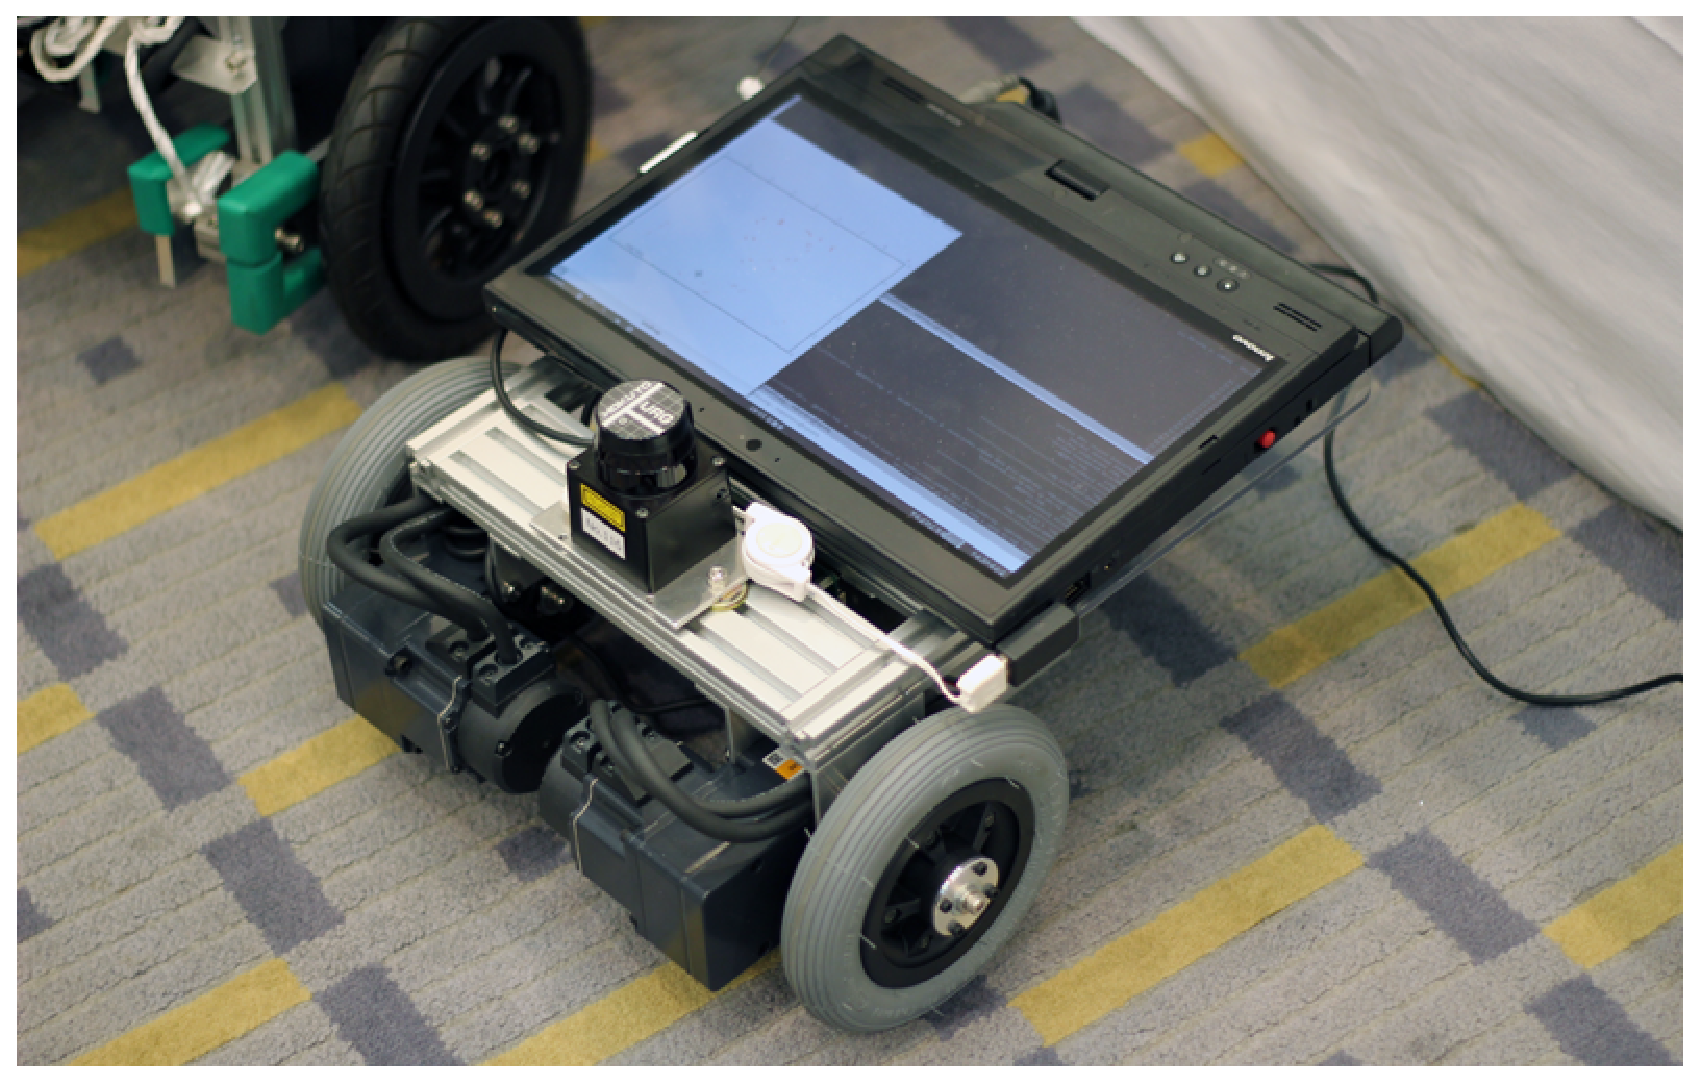
\includegraphics[width=90mm]{icart-mini.eps}
\caption{差動駆動型移動ロボットの例}
\label{fig:example_robot}
\end{figure}

 本モータドライバは、産業用ロボットなどで広く用いられている、ブラシレスモータ(ACサーボモータ)の駆動・制御に対応しています。
また、モータの特性やロボットのダイナミクスを考慮した、フィードフォワード制御を活用できるため、高い制御性を実現できます。\par

\subsection{T-frogプロジェクト}
 2010年に、筑波大学知能ロボット研究室の移動ロボット技術の移転と利用の促進のため、筑波大学と茨城県内の中小企業などをメンバーとして、T-frog ({\bf{F}}uture~{\bf{Ro}}botics~{\bf{G}}roundworks~from~{\bf{T}}sukuba)プロジェクトが発足しました。
本モータドライバは、T-frogプロジェクトの一環として開発されたモジュールです。\par

{\bf TF-2MD3-R6}は、ツジ電子株式会社
\footnote{\makebox[10em][l]{ツジ電子株式会社} 〒300-0013 茨城県土浦市神立町3739、info2[at]tsuji-denshi.co.jp、029-832-3031}
と渡辺敦志
\footnote{\makebox[10em][l]{渡辺敦志} 筑波大学知能ロボット研究室(2013年度現在)、atsushi.w[at]ieee.org}
を中心に開発しています。
また、本モータドライバモジュールには、筑波大学知能ロボット研究室
\footnote{\makebox[10em][l]{知能ロボット研究室} 〒305-8573 茨城県つくば市天王台1-1-1 筑波大学 システム情報工学研究科、029-853-5155}
の研究成果が用いられています。\par


\newpage
% ---------------------------------------------------------------------
% --------------------------- subsection ------------------------------
\subsection{主な仕様}
\label{sec:主な仕様}

{\bf TF-2MD3-R6}の外観を\figurename~\ref{fig:driver_board_r6} に、主な仕様を\tablename~\ref{tb:tfrog_motor_driver} に示します。
本モータドライバは1台につき、ブラシレスモータまたはDCモータを2台駆動・制御できます。
通信インタフェースはUSBのCDC-ACMクラスに対応しており、Linux、Mac OS X、Windows環境で使用可能(Windows環境ではドライバが必要)です。
通信プロトコルは筑波大学 知能ロボット研究室で開発している移動ロボット走行制御ソフトウェアプラットフォーム {\bf YP-Spur} \footnote{Robot Platform Project \\ \hspace{2em}{\scriptsize\url{http://www.roboken.iit.tsukuba.ac.jp/platform/}}}と互換性があります。\par

\begin{figure}[H]
\centering\includegraphics[width=120mm]{driver_board_r6.eps}
\caption{{\bf TF-2MD3-R6}の外観}
\label{fig:driver_board_r6}
\end{figure}

\begin{table}[H]
\caption{{\bf TF-2MD3-R6}の主な仕様}
\label{tb:tfrog_motor_driver}
\smallskip
\centering\begin{tabular}{rl}
\toprule
対応モータ			&	3相 ブラシレスモータ			\\*[-1mm]
					&	DCモータ						\\
モータ数			&	2台								\\
インタフェース		&	USB2.0 (CDC-ACM)				\\*[-1mm]
					&	UART (3.3~V \ CMOS)				\\*[-1mm]
					&	RS-485							\\
最大電源電圧		&	12--50~V						\\
最大連続電流		&	5~A/ch (自然空冷)				\\
PWM分解能			&	1200 (20~kHz時)					\\
エンコーダ入力		&	2相 パルスエンコーダ			\\*[-1mm]
					&	3相 ホール素子+原点信号			\\
寸法				&	100~x~55~x~30~mm				\\
重量				&	100~g							\\
その他				&	AD変換(3.3V) 7~ch、デジタルIO(3.3V) 8~ch	\\
\bottomrule
\end{tabular}
\end{table}


\newpage
% ---------------------------------------------------------------------
% --------------------------- subsection ------------------------------
\subsection{{\bf TF-2MD3-R6}を用いた移動ロボットのシステム構成}
\label{sec:システム構成}

{\bf TF-2MD3-R6}と、{\bf YP-Spur} を用いた移動ロボット走行制御システムの構成を、\figurename~\ref{fig:yp-system} に示します。
本モータドライバは、\figurename~\ref{fig:yp-system} 下部の ``モータドライバユニット'' 部分に相当します。
モータドライバ上のマイクロコンピュータでは、ラップトップコンピュータから送信された制御パラメータを用いて、速度制御の目標値に追従するように、モータの角速度をPI制御します。PI制御器には、車輪を駆動したときに、独立二輪躁舵(差動駆動)型移動ロボットの動特性によって他の車輪に及ぼす影響などを補償するためのフィードフォワード補償器\cite{the:pws_ff_cnt}\cite{the:vehicle_control}が内蔵されています。\par
\begin{figure}[H]
\centering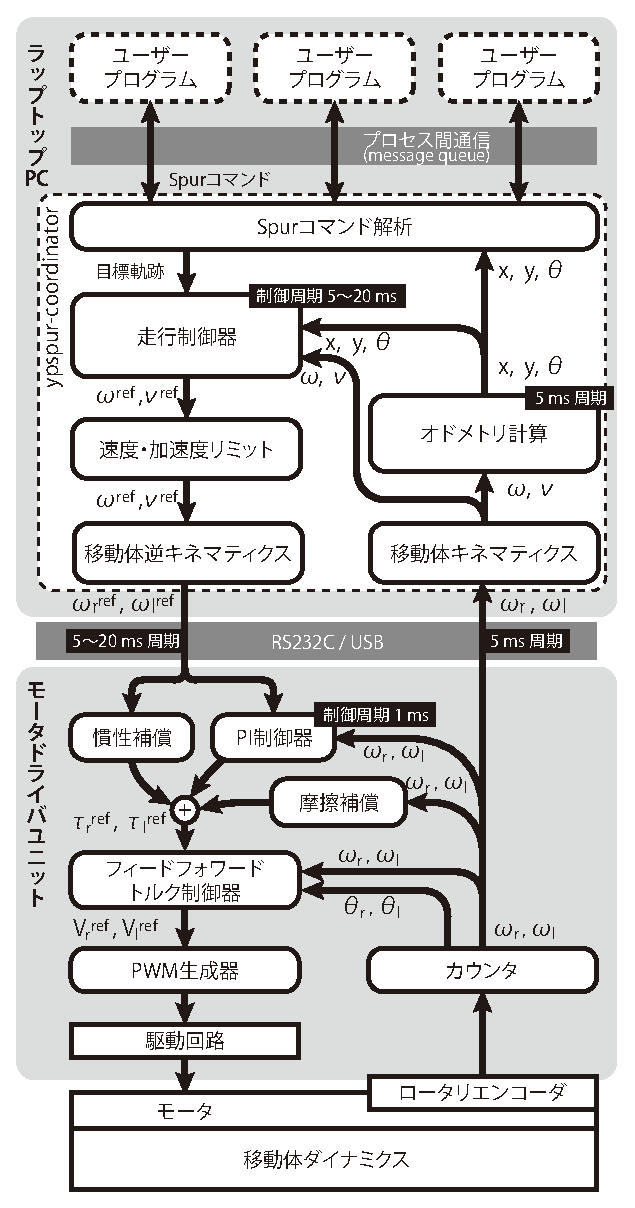
\includegraphics[width=90mm]{system2.eps}
\caption{{\bf TF-2MD3-R6}と{\bf YP-Spur} を用いた移動ロボット走行制御システムの構成}
\label{fig:yp-system}
\end{figure}


\newpage
% ******************************************************************
% **************************** section *****************************
\section{取り扱い上の注意}
\label{sec:取り扱い上の注意}

% ---------------------------------------------------------------------
% --------------------------- subsection ------------------------------
\subsection{注意}
\label{sec:注意}

けがや、機器の故障を防ぐために、以下の事項を必ずご確認下さい。\par

\warnbox{電源ケーブル・コネクタは}{
	\iconitem{warn.eps}{
		\item ピン配置が正しいことを確認する
		\item 正しく圧着できていることを確認する
		\item 駆動するモータの合計容量に見合った定格容量を確保する
	}
}

\warnbox{モータ・エンコーダのケーブル・コネクタは}{
	\iconitem{warn.eps}{
		\item ピン配置が正しいことを確認する
		\item モータとエンコーダの組み合わせが正しいことを確認する
	}
}

\warnbox{本製品への電源供給は}{
	\iconitem{warn.eps}{
		\item モータ駆動電源には、使用する動作範囲を考慮してヒューズまたはブレーカーを挿入する
		\item モータ駆動電源のケーブルはできるだけ短くし、過電圧保護回路または、低ESRの大容量キャパシタを挿入する (\ref{sec:電源の供給}~参照)
		\item 5V電源には、100mA$\sim$1A程度のヒューズまたはブレーカーを挿入する
	}
}

\warnbox{異常を感じたときは}{
	\iconitem{warn.eps}{
		\item 正しく動作しなくなったら、事故防止のためすぐに電源を切る
		\item 基板が発熱していないことを確認する
		\item 電流制限機能付きの電源装置から電源を供給し、動作を確認する
		\item 異常が続くときは、開発者へ問い合わせる
	}
}

\warnbox{動作中の製品には}{
	\iconitem{donot.eps}{
		\item 基板に直接手を触れない(人体の寄生容量や静電気による誤動作を防ぐため)
		\item コネクタを着脱しない
	}
}

\warnbox{走行制御プログラムの起動時には}{
	\iconitem{warn.eps}{
		\item パラメータファイルが正しいことを確認する
	}
	\itemseprule
	\iconitem{donot.eps}{
		\item モータで駆動する部分に手を置かない
	}
}


% ---------------------------------------------------------------------
% --------------------------- subsection ------------------------------
\subsection{推奨事項}
\label{sec:推奨}

製品の正常な動作のために、以下の事項を推奨致します。
\par
\null


\warnbox{通信インタフェースには}{
	\iconitem{recommend.eps}{
		\item シールド付きのUSBケーブルを使用する
		\item ノイズが多い環境などで通信が切断される場合は、フェライトコア付きのUSBケーブルを使用する
	}
}

\warnbox{本製品への電源供給は}{
	\iconitem{recommend.eps}{
		\item モータ駆動電源の電圧変動が、5V電源に伝わりにくいように構成する
	}
}

\warnbox{ソフトウェアについて}{
	\iconitem{recommend.eps}{
		\item {\bf TF-2MD3-R6}のファームウェア更新、{\bf YP-Spur} のソフトウェア更新を確認し、バグ修正などがあった際は更新する
	}
}



\newpage
% ---------------------------------------------------------------------
% --------------------------- subsection ------------------------------
\subsection{免責事項}
\label{sec:免責}

T-frogプロジェクトは、T-frogプロジェクトの製品及びサービスを任意に修正、改善、改良、およびその他の変更をし、製品の製造およびサービスの提供を中止する権利を留保します。
製品を発注される前には、関連する最新の情報を取得して頂き、その情報が現在有効かつ完全なものであることをご確認下さい。
\par

T-frogプロジェクトは、T-frogプロジェクトの製品を使用したお客様の製品設計および、アプリケーションに関する支援について、責任を負いません。
T-frogプロジェクトの製品を使用した、お客様の製品およびアプリケーションについての責任はお客様にあります。
T-frogプロジェクトの製品を使用した、お客様の製品およびアプリケーションの安全対策は、必ずお客様にてお取り下さい。
\par

T-frogプロジェクトの製品は、移動ロボット研究用途に使用することを想定して、設計、および製造されています。
T-frogプロジェクトは、T-frogプロジェクトの製品が安全でないことが致命的となる用途 (例えば、生命維持装置のように、T-frogプロジェクトの製品に不具合があった場合に死傷などの重篤な事故が発生するもの) に使用されることを認めません。
また、T-frogプロジェクトの製品は、自動車用アプリケーション、軍事的用途、もしくは航空宇宙アプリケーションで使用されるようには設計されておらず、使用されることを意図していません。
お客様は、T-frogプロジェクトの製品を、自動車の環境、軍事的環境、または航空宇宙環境で使用することは、お客様の危険負担においてなされること、および、お客様の責任をもって、それらの用途に必要な全ての法的要求事項および規制上の要求事項を満足させなければならないことを認め、かつ同意します。
\par



\newpage
% ******************************************************************
% **************************** section *****************************
\section{{\bf TF-2MD3-R6}の接続と取り付け}
\label{sec:モータドライバの接続}

% ---------------------------------------------------------------------
% --------------------------- subsection ------------------------------
\subsection{コネクタ・ピン配置}
\label{sec:コネクタ}

{\bf TF-2MD3-R6}使用時には、モータドライブ用電源、コントローラ用電源、モータ、エンコーダ、USBコネクタを接続します。
各コネクタの配置と、適合するハウジング・コンタクト品番を\figurename~\ref{fig:connector6} に示します。
\par

\begin{figure}[H]
\centering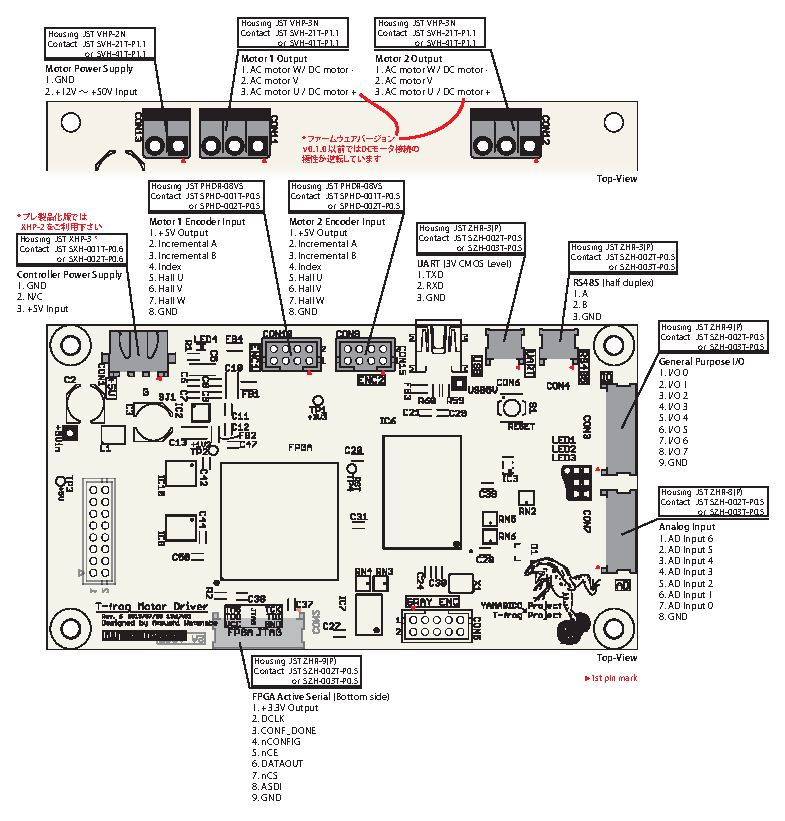
\includegraphics[width=160mm]{pin-description-r6.eps}
\caption{{\bf TF-2MD3-R6}のコネクタ・ピン配置}
\label{fig:connector6}
\end{figure}

ブラシレスモータのU端子に対して、V端子、W端子にそれぞれ120度、240度遅れた波形の3相交流を印加したときの回転方向、またはDCモータの+端子に正電圧を印加したときの回転方向において、エンコーダのA相立ち上がりから90度遅れて、B相が立ち上がるように接続して下さい。
\par


% ---------------------------------------------------------------------
% --------------------------- subsection ------------------------------
\subsection{電気的特性}
\label{sec:電気的特性}

{\bf TF-2MD3-R6}の、各コネクタの絶対最大定格を\tablename~\ref{tb:abs_max6} に示します。絶対最大定格を超えた電圧が一瞬でも印加されると、モータドライバが破損する可能性があります。
また、電気的特性を\tablename~\ref{tb:el_char6} に示します。
モータドライブ用電源およびモータのコネクタ(JST VHシリーズ)の定格連続電流は10Aですので、これ以上の電流が必要な場合は、ケーブルを直接半田付けするか、基板に端子台などを取り付けて配線して下さい。\par

\begin{table}[H]
%\begin{minipage}[t]{0.44\hsize}
\caption{{\bf TF-2MD3-R6} 絶対最大定格}
\label{tb:abs_max6}
\centering\begin{tabular}{rl}
\toprule
コントローラ基板電源 & -0.5 $\sim$ +7~V \\
モータドライブ電源 & -0.5 $\sim$ +60~V \\
\midrule
エンコーダ入力 & -0.5 $\sim$ +7~V \\
\bottomrule
\end{tabular}
%\end{minipage}
\end{table}

\begin{table}[H]
%\begin{minipage}[t]{0.54\hsize}
\caption{{\bf TF-2MD3-R6} 電気的特性}
\label{tb:el_char6}
\centering\begin{tabular}{rl}
\toprule
コントローラ基板電源 & 4.5 $\sim$ 5.5~V \\
モータドライブ電源 & +10 $\sim$ 50~V \\
\midrule
エンコーダ入力プルアップ & 4.7~k$\Omega$ \\
エンコーダ入力LOレベル閾値 & 0.6~V \\
エンコーダ入力HIレベル閾値 & 2.2~V \\
\midrule
コントローラ基板電流 & typ 140~mA {\footnotesize(1} \\
ドライブ基板スタンバイ電流 & typ 20~mA \\
\bottomrule
\end{tabular}
%\end{minipage}
\begin{center}
{\footnotesize\centering (1 エンコーダなどの電流を除く、USB通信時。}
\end{center}
\end{table}

\newpage
% ---------------------------------------------------------------------
% --------------------------- subsection ------------------------------
\subsection{電源の供給}
\label{sec:電源の供給}

誘導性の負荷(モータ)を駆動中に電源が遮断され、電源端子が開放されると、誘導電流によりモータドライバが破損する場合があります。
これを防ぐため、モータ駆動電源のケーブルはできるだけ短くし、可能な限りモータドライバから近い位置(5cm以内を推奨)に低ESRのキャパシタを挿入して下さい。
\par
駆動中に電源が遮断された際に、回路の保護に必要なキャパシタ容量$C_{p}$は以下を参考に算出して下さい。
\par

\begin{itemize}
\setlength{\leftskip}{30pt}
%\item [$R_{m}$] モータ端子間抵抗 [$\Omega$]
\item [$L_{m}$] モータ端子間インダクタンス [H]
\item [$E_{p}$] 電源電圧 [V]
\item [$I_{max}$] 瞬間最大電流 [A]
\end{itemize}

%モータに流れうる最大の電流(最大回転数の状態で逆方向に最大電圧で駆動した際の電流 $2E_{p}/R_{m}$)によって、モータのインダクタンスに蓄えられるエネルギー$P_{l}$は、次式で求められます。
%モータに流れうる瞬間最大電流$I_{max}$によって、モータのインダクタンスに蓄えられるエネルギー$P_{l}$は、次式で求められます。
%\begin{eqnarray*}
%P_{l} = \frac{1}{2} L_{m} I_{max}^{2}
%\end{eqnarray*}
\figurename~\ref{fig:circuit_cap}に示す回路構成において、モータドライバの保護に必要なキャパシタ容量は次式で算出できます。
\begin{eqnarray*}
C_{p} > 2 \frac{L_{m} I_{max}^{2}}{60^2 - E_{p}^{2}}
\end{eqnarray*}

\begin{figure}[H]
\centering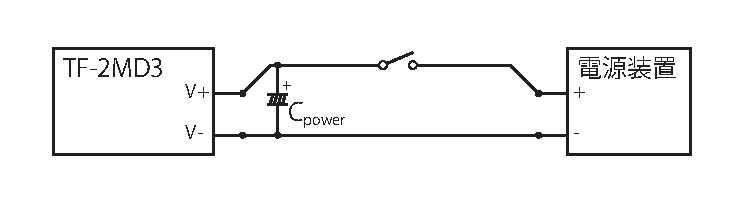
\includegraphics[width=100mm]{circuit_cap.eps}
\caption{電源供給回路の構成}
\label{fig:circuit_cap}
\end{figure}

例えば、インダクタンス$L_{m}=1.5$~[mH]、抵抗$R_{m}=0.8$~[$\Omega$]のモータを、電源電圧$E_{p}=24$~[V]で使用する場合(ブラシレスモータ TF-M30-24-3500-G15L/R 相当)、以下のキャパシタ容量が必要になります。
(瞬間最大電流$I_{max}$を、パラメータ誤りなどで制御系が暴走してロックした状態のモータに最大出力を与えた際の電流 $I_{max}=E_{p}/R_{m}=24/0.8=30.0$とした場合\footnote{なお、TF-M30-24-3500-G15L/Rに$30$[A]の電流が流れた場合、モータは減磁、破損します。})
\begin{eqnarray*}
%P_{l} &=& \frac{1}{2} 0.0015 \cdot 30^{2} = 0.675 \text{[J]}\\
C_{p} &>& 2 \frac{0.0015 \cdot 30^{2}}{60^{2} - 24^{2}} = 0.00089 \text{[F]} = 890 \text{[uF]}
\end{eqnarray*}
ただし、キャパシタ容量のばらつきや、温度による容量変化、電源電圧の変動などを加味して、十分な安全率をとる必要があります。


ZNR素子や専用IC等の、過電圧保護回路を組み込むことで必要な容量を削減できる場合があります。その際に必要なキャパシタ容量は、構成に応じて別途算出して下さい。


\ovalbox{
\begin{minipage}[l]{0.95\textwidth}
\vspace{0.8em}
{\bf\large 参考資料: $C_{p}$の導出}\\
\parbox{\textwidth}{
\vspace{0.5em}
\parindent=1em
容量$C$のキャパシタの端子間電圧が$E$のとき、キャパシタに蓄えられているエネルギー$P$は次式で求まる。
\begin{eqnarray*}
 P = \frac{1}{2} C \cdot E^{2}
\end{eqnarray*}
モータドライバ動作中はキャパシタは電源電圧$E_{p}$で充電されている。
この状態で電源が切断されると、モータ2台のインダクタンスに蓄えられているエネルギー$2P_{l}$がキャパシタに回生される。その際の、キャパシタの総エネルギー$P_{c}$は次式で表される。
\begin{eqnarray*}
 P_{c} = \frac{1}{2} C_{p} \cdot E_{p}^{2} + 2P_{l}
\end{eqnarray*}
このときのキャパシタ電圧$E_{c}$と容量$C_{p}$の関係は次式で表される。
\begin{eqnarray*}
 P_{c} &=& \frac{1}{2} C_{p} \cdot E_{c}^{2}\\
 \frac{1}{2} C_{p} \cdot E_{p}^{2} + 2P_{l} &=& \frac{1}{2} C_{p} \cdot E_{c}^{2}
\end{eqnarray*}
\par

モータドライバが破損しないためには、キャパシタの電圧が、モータドライバの絶対最大定格電圧$E_{max}$以下であればよい。
したがって、モータドライバがモータの誘導電流によって破壊されない最小のキャパシタ容量$C_{p}$は次式で求まる。
\begin{eqnarray*}
 \frac{1}{2} C_{p} \cdot E_{p}^{2} + 2P_{l} &=& \frac{1}{2} C_{p} \cdot E_{max}^{2}\\
 C_{p} &=& 2\frac{2P_{l}}{E_{max}^{2} - E_{p}^{2}}
\end{eqnarray*}
}
\end{minipage}
\vspace{0.8em}
}


\newpage
% ---------------------------------------------------------------------
% --------------------------- subsection ------------------------------
\subsection{外形と取り付け穴}
\label{sec:外形と取り付け穴}

{\bf TF-2MD3-R6}の外形図と取り付け穴の配置を\figurename~\ref{fig:shape} に示します。
基板は2枚構成で、上部をコントローラ基板、下部をドライブ基板と呼びます。
コントローラ基板とドライブ基板は基板スペーサで取り付けてあります。
ドライブ基板の裏面には基板スペーサ(10mm高)が取り付けられており、M3.0のネジで固定できます。

\begin{figure}[H]
\centering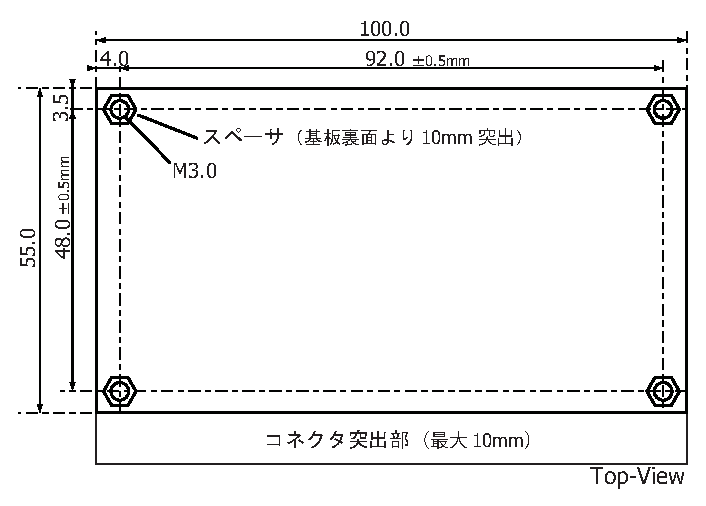
\includegraphics[width=130mm]{shape_r6.eps}
\caption{{\bf TF-2MD3-R6}の外形図}
\label{fig:shape}
\end{figure}



\newpage
% ******************************************************************
% **************************** section *****************************
\section{{\bf YP-Spur} を用いたロボット制御}
\label{sec:YP-Spur}

{\bf TF-2MD3-R6}は、移動ロボット走行制御ソフトウェアプラットフォーム ``{\bf YP-Spur} '' の通信仕様に対応しています。
{\bf TF-2MD3-R6}と{\bf YP-Spur} を組み合わせて用いることで、容易に移動ロボットの走行制御系を構築できます。
\par

{\bf YP-Spur} は、Unix互換のシステム(Linux、Mac OS Xなど)、およびWindowsで動作します。
Mac OS Xでは、アタッチされるデバイスのパスなどが異なります。
Unix互換のシステムで用いる場合、バージョン管理ツールgit、およびgcc+glibcまたは、それらに相当する開発環境がインストールされている必要があります。\par

動作確認には、ロボットのパラメータファイルが必要となります。
T-frogプロジェクトのオープンソースロボットハードウェア ``i-Cart mini'' のパラメータファイルは、\url{http://t-frog.com/products/icart_mini/} からダウンロードできます。
新規に作成したロボットのパラメータは、\ref{sec:パラメータ作成}章を参考に作成して下さい。\par

% ---------------------------------------------------------------------
% --------------------------- subsection ------------------------------
\subsection{開発環境の構築と動作テスト: Linux}

以下のコマンドで、コンパイル環境とバージョン管理ツールをインストールします。

{\bf Ubuntuの場合}
\begin{lstlisting}{}
$ sudo apt-get update
$ sudo apt-get install build-essential libreadline-dev
$ sudo apt-get install git git-svn
\end{lstlisting}

{\bf Fedoraの場合}
\begin{lstlisting}{}
$ sudo yum groupinstall "Development Tools"
$ sudo yum install readline-devel
$ sudo yum install git git-svn
\end{lstlisting}


{\bf YP-Spur} を、以下のコマンドでインストールします。\par
\begin{lstlisting}{}
$ git clone https://openspur.org/repos/yp-spur.git/
$ cd yp-spur
$ ./configure
$ make
$ sudo make install
$ sudo ldconfig
$ cd ..
\end{lstlisting}


{\bf YP-Spur} を用いたロボットの走行制御は、ラップトップPC上で走行制御を行う ``ypspur-coordinator'' プロセスと、ユーザプログラムのプロセスを動作させることで行います。
1.0 x 0.1 メートルの四角形を描くように走行する、{\bf YP-Spur} のサンプルプログラムを実行するには、ターミナルを2つ開き、それぞれで以下のコマンドを実行します。

\warnbox{YP-Spurサンプルプログラムの起動時には}{
	\iconitem{warn.eps}{
		\item パラメータファイルが正しいことを確認する
		\item ロボットの正面1.5メートル、左右1メートル程度の空間を確保して実行する
	}
}

{\bf 1つ目のターミナルで実行}
\begin{lstlisting}{}
$ ypspur-coordinator -p PARAMETER_FILE.param -d DEVICE_PATH
\end{lstlisting}

{\bf 2つ目のターミナルで実行}
\begin{lstlisting}{}
$ cd yp-spur/samples/
$ ./run-test
\end{lstlisting}

コマンド中の PARAMETER\_FILE.param には、ロボットのパラメータファイルへのパスを指定します。
{DEVICE\_PATH} は、{/dev/ttyACM0} のように Linux 上にアタッチされるデバイスのフルパスを指定します。

\newpage
% ------------------------ subsubsection ------------------------------
\subsection{開発環境の構築と動作テスト: Windows}

下記URLから、{\bf TF-2MD3-R6}の Windows 用のデバイスドライバをダウンロード、解凍し、``setup.bat''を右クリック、``管理者として実行''して下さい。
PCに{\bf TF-2MD3-R6} を接続する前に予め、ドライバをインストールして下さい。
(Windows 8 以降では、署名無しのドライバインストールを許可する設定が必要です。)\\
\urllink{http://t-frog.com/products/motor_driver/}
\par

{\bf YP-Spur} を、下記のURLからダウンロードし、展開します。
MinGW、Cygwin環境で使用する場合は、展開したファイルをMinGW、Cygwin環境のルートディレクトリなどにコピーし、Linuxの場合を参考に動作テストを行って下さい。
lib ディレクトリ下のライブラリ、DLLファイル、および include ディレクトリ下のヘッダファイルを使用することで、Microsoft Visual C++ を用いた開発が可能です。\\
\urllink{https://openspur.org/ypspur_downloads.php}
\par

{\bf YP-Spur} を用いたロボットの走行制御は、ラップトップPC上で走行制御を行う ``ypspur-coordinator'' プロセスと、ユーザプログラムのプロセスを動作させることで行います。
1.0 x 0.1 メートルの四角形を描くように走行する、{\bf YP-Spur} のサンプルプログラムを実行するには、以下の手順を行って下さい。
\begin{enumerate}
\item 展開したファイルの bin ディレクトリ中の ypspur-gui.exe を実行する
\item Browse ボタンで、ロボットのパラメータファイルを開く
\item Port 欄で、モータドライバのデバイス名を選択する
\item Start/Stop ボタンを選択し、エラー表示が発生していないことを確認する
\item 上記URLから別途、run-test.exe をダウンロードし、実行する
\end{enumerate}

\warnbox{YP-Spurサンプルプログラムの起動時には}{
	\iconitem{warn.eps}{
		\item パラメータファイルが正しいことを確認する
		\item ロボットの正面1.5メートル、左右1メートル程度の空間を確保して実行する
	}
}

\newpage
% ******************************************************************
% **************************** section *****************************
\section{{\bf YP-Spur} ロボットパラメータ}
\label{sec:ロボットパラメータ}

{\bf TF-2MD3-R6}は、DCモータ・ブラシレスモータに対応しており、モータの種類などの情報を{\bf YP-Spur} のロボットパラメータファイルで指定する必要があります。
詳細なパラメータ決定方法・調整方法はYP-SpurリポジトリのWiki\footnote{YP-Spurリポジトリ Wiki \\ \hspace{2em}{\scriptsize\url{https://github.com/openspur/yp-spur/wiki/}}}を参照して下さい。\par

% ---------------------------------------------------------------------
% --------------------------- subsection ------------------------------
\subsection{ブラシレスモータ用のロボットパラメータ作成}
\label{sec:パラメータ作成}

モータ種別の指定は MOTOR\_PHASE 項で行い、DCモータの場合は0を、3相ブラシレスモータの場合は3を指定します。
ブラシレスモータを使用する場合は、内部抵抗・逆起電力係数・トルク係数は、DCモータに換算した値を指定します。
\begin{itemize}
\item {\bf MOTOR\_R: モータ内部抵抗[$\Omega$]} \par モータの端子間抵抗$R$から、$\frac{3}{4} \cdot R$で与える
\item {\bf MOTOR\_VC: 逆起電力係数[rpm/V]} \par 定格電圧$V$でのモータ無負荷最大回転数$r_{max}$から、$r_{max}/V$で与える
\item {\bf MOTOR\_TC: トルク係数[Nm/A]} \par 逆起電力係数$K_{E}=r_{max}/V$から単位を変換し、$\frac{60}{2\pi K_{E}}$で与える\footnote{モータのエネルギー損失が無視できる場合、モータに注入した電力$P = E \cdot I = K_{E} \cdot \omega \cdot I$と、モータが発する動力$P = \tau \cdot \omega = K_{\tau} \cdot I \cdot \omega$が釣り合うため、$K_{E} = K_{\tau}$が成り立つ(単位系に注意)}
\end{itemize}\par

また、ブラシレスモータが、n極(モータ軸を1回転すると逆起電力波形やホール素子波形がn周期現れる)場合は、ギア比(GEAR 項)をn倍し、エンコーダ分解能(COUNT\_REV 項)を1/nとする必要があります。モータ軸の慣性モーメントを指定する MOTOR\_M\_INERTIA 項 はギア比がn倍だった場合に換算して指定する必要があるので、モータ軸の慣性モーメント$M$に対して、$M/n^{2}$を与えます。\par

{\bf TF-2MD3-R6}と{\bf YP-Spur} を用いて、パラメータを適切に設定すれば、フィードフォワード制御によりロボット走行制御の特性を向上できます。\par


% ---------------------------------------------------------------------
% --------------------------- subsection ------------------------------
\subsection{パラメータファイル作成例}
\label{sec:パラメータ作成例}

最小構成の移動ロボットは、{\bf TF-2MD3-R6}の他に、モータ・タイヤ・電源・ラップトップPCがあれば構築できます。
\figurename~\ref{fig:simple_robot} に、{\bf TF-2MD3-R6}の動作テスト用に構築した簡易な移動ロボットを示します。オリエンタルモータのブラシレスモータ(BX230A-15FRにパルスエンコーダを取り付けたバージョン)を搭載し、ダイレクトドライブでタイヤを駆動する構成となっています。\par
このときの、パラメータファイルの主要な部分を以下に示します。このモータは3相5極なので、ギア比は5倍となっています。\par
\begin{figure}[H]
\centering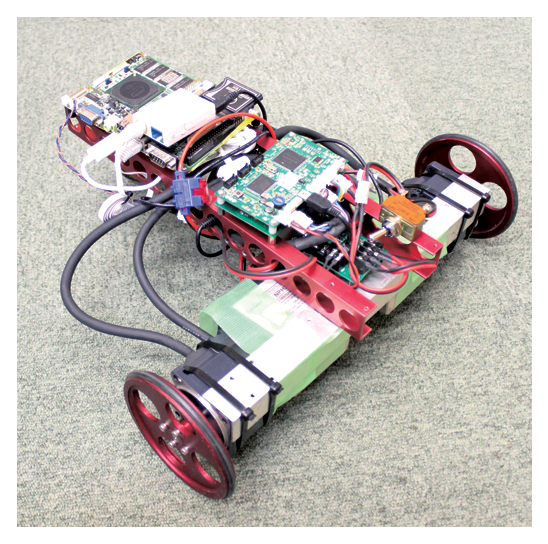
\includegraphics[width=65mm]{simple_robot.eps}
\caption{ブラシレスモータを用いたダイレクトドライブ移動ロボットの例}
\label{fig:simple_robot}
\end{figure}


\begin{lstlisting}{}
     MOTOR_PHASE    3.00000000 #
 TORQUE_FINENESS    0.00000100 #
       COUNT_REV  400.00000000 #[cnt/rev]
            VOLT   24.00000000 #[V]
           CYCLE    0.00100000 #[s]
            GEAR    5.00000000 #[in/out]
         MOTOR_R    0.80000000 #[ohm]
        MOTOR_TC    0.01527887 #[Nm/A]
        MOTOR_VC  600.00000000 #[rpm/V]

       RADIUS[0]   -0.05600000 #[m]
       RADIUS[1]    0.05600000 #[m]
           TREAD    0.39000000 #[m]
   CONTROL_CYCLE    0.02000000 #[s]
         GAIN_KP   35.00000000 #P gain
         GAIN_KI   45.00000000 #I gain
      TORQUE_MAX    0.40000000 #[Nm]
    TORQUE_LIMIT    0.50000000 #[Nm]
   TORQUE_NEWTON    0.00200000 #[Nm]
   TORQUE_VISCOS    0.00000000 #[Nm/rad/s]

         MAX_VEL    3.00000000 #[m/s]
           MAX_W    6.28000000 #[rad/s]
       MAX_ACC_V    2.00000000 #[m/ss]
       MAX_ACC_W   12.50000000 #[rad/ss]
  MAX_CENTRI_ACC    2.45000000 #0.25G

    INTEGRAL_MAX    0.20000000 #[rev]
            MASS    5.00000000 #[kg]
  MOMENT_INERTIA    0.10000000 #[kgm^2]
 MOTOR_M_INERTIA    0.00000093 #[kgm^2]
  TIRE_M_INERTIA    0.00300000 #[kgm^2]
\end{lstlisting}


\newpage
% ******************************************************************
% **************************** section *****************************
\section{{\bf TF-2MD3-R6}のファームウェア更新方法}
\label{sec:ファームウェア更新方法}

{\bf TF-2MD3-R6}のファームウェア更新は、USBインタフェースで行います。

\warnbox{ファームウェアの更新時}{
	\iconitem{donot.eps}{
		\item 作業中は、モータ駆動電源を供給しない
		\item 作業を中断しない
	}
}

基板のバージョンと一致するコンパイル済みのファームウェアを、以下のURLからダウンロードします。
ソースコードをダウンロードしてコンパイルすることでも生成できます。\\
\urllink{http://t-frog.com/products/motor_driver/}

% ---------------------------------------------------------------------
% --------------------------- subsection ------------------------------
\subsection{Linux環境の場合}
\label{sec:Linuxファームウェア}


以下のコマンドで、 ``samba Flash Utility for AT91SAM7 microcontrollers''、および書き込みスクリプトをインストールします。
\begin{lstlisting}{}
$ git clone https://github.com/at-wat/samba.git
$ cd samba
$ ./configure
$ make
$ sudo make install
$ cd ../
$ git clone https://github.com/T-frog/tf2md3_flash.git
$ cd tf2md3_flash
$ sudo make install
\end{lstlisting}
\par

%はじめに、以下のコマンドを実行して、{FLASH~ROM} を消去します。 
%{DEVICE\_PATH} には、 {/dev/ttyACM0} のように Linux 上にアタッチされたデバイスのフルパスを指定します。
%\begin{lstlisting}{}
%$ echo '$FLASHERACEA' > DEVICE_PATH
%$ echo '$FLASHERACEB' > DEVICE_PATH
%\end{lstlisting}
%\par
%
%{\bf TF-2MD3-R6} をUSBインタフェースでコンピュータに接続、コントローラ基板電源(5V)を投入し、
以下のコマンドを実行します。
{DEVICE\_PATH} は、{/dev/ttyACM0} のように Linux 上にアタッチされるデバイスのフルパスを指定し、
FIRMWARE.bin はコンパイル済みのファームウェアのパスを指定します。
%\begin{lstlisting}{}
%$ samba -i DEVICE_PATH
%> flash 0x00100000 FIRMWARE.bin
%> nvm 4
%\end{lstlisting}
\begin{lstlisting}{}
$ tf2md3_flash DEVICE_PATH FIRMWARE.bin
\end{lstlisting}
作業が完了したら、コントローラ基板電源を切断し、再度、投入します。

\bigskip
\warnbox{ハードウェアスイッチで消去した場合、書き込みを中断した場合の書き込み}{
	\iconitem{warn.eps}{
		\item ハードウェアスイッチでファームウェアを消去した場合、書き込みを途中で中断して再度書き込む場合は、以下のコマンドを使用して下さい\\
{\tt \$ tf2md3\_flash DEVICE\_PATH FIRMWARE.bin --erased}
	}
}
\warnbox{ファームウェア更新成功の確認}{
	\iconitem{warn.eps}{
		\item 電源投入時に、LED1が短時間点灯した後消灯、LED2が薄く点灯することを確認する
	}
}


\newpage
% ---------------------------------------------------------------------
% --------------------------- subsection ------------------------------
\subsection{Windows環境の場合}
\label{sec:Windowsファームウェア}

``SAM-BA 2.** for Windows'' を下記のURLからダウンロードし、インストールします。)(3.*.*シリーズは本製品に対応していません。)\\
\urllink{http://www.atmel.com/tools/ATMELSAM-BAIN-SYSTEMPROGRAMMER.aspx}
\par


{\bf TF-2MD3-R6}をUSBインタフェースでコンピュータに接続、コントローラ基板電源(5V)を接続します。
はじめに、{Tera~Term} {\small(\url{http://sourceforge.jp/projects/ttssh2/})}  などのターミナルソフトウェアで、{\bf TF-2MD3-R6} のCOMポートを開き、受信改行コードの設定を``LF''に、送信改行コードの設定を``LF''または``CR+LF''に変更します。
以下のコマンドを入力してFLASH ROMを消去します。(先頭の``\$''も入力して下さい。)
\begin{lstlisting}{}
$FLASHERACEA
$FLASHERACEB
\end{lstlisting}
入力中は文字列は表示されませんが、入力後に下記の表示が現れます。
\begin{lstlisting}{}
$FLASHERACEA
00P

$FLASHERACEB
00P

\end{lstlisting}
\par


表示が異なる場合は、ターミナルソフトウェアを終了してから、コントローラ基板電源を切断、再度接続し、上記の手順をやり直して下さい。


なお、初回接続時には、デバイスドライバのインストールウィザードが開きますので、画面の指示に従ってデバイスドライバをインストールして下さい。
Windows~7の場合は、以下の手順でインストールできます。
\begin{enumerate}
	\item スタートボタンの ``コントロールパネル'' から、 ``システム'' を開き、 ``デバイスマネージャ'' を選択
		\begin{figure}[H]
			\centering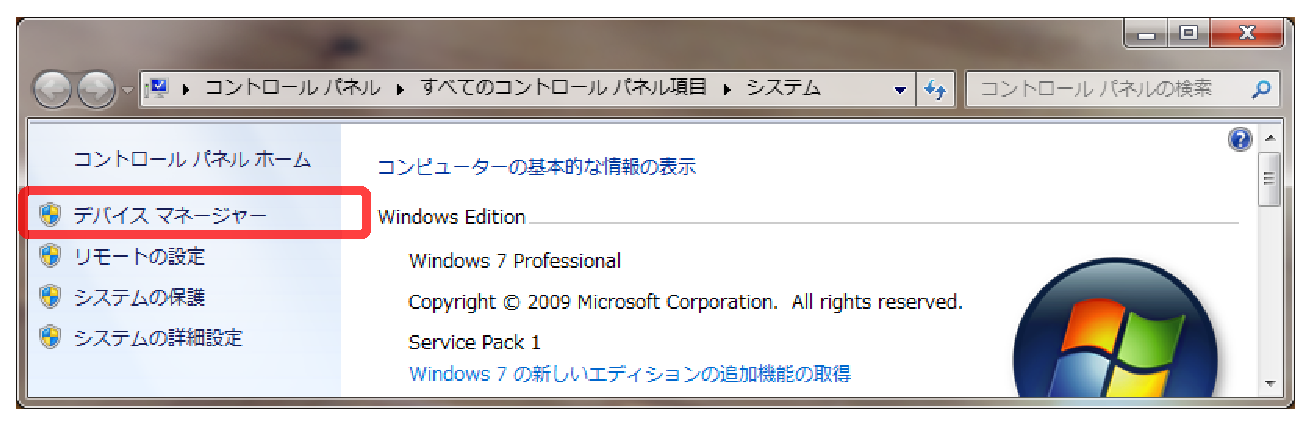
\includegraphics[width=122mm]{windriver-install.3.system.eps}
			\caption{デバイスマネージャを起動}
			\label{fig:windriver.system}
		\end{figure}
	\item ``ほかのデバイス'' を展開し、 ``不明なデバイス'' を右クリック、 ``プロパティ'' を選択
		\begin{figure}[H]
			\centering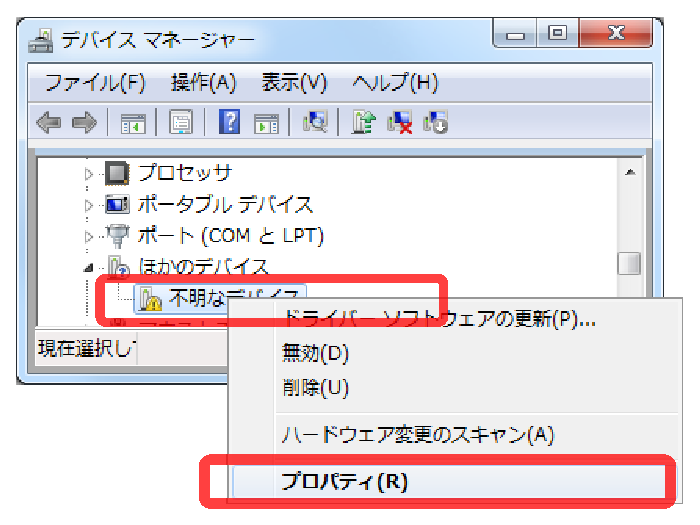
\includegraphics[width=64mm]{windriver-install.4.device_man.eps}
			\caption{不明なデバイスのプロパティを開く}
			\label{fig:windriver.device_man}
		\end{figure}
	\item ``ドライバー'' タブの ``ドライバーの更新(P)'' を選択
		\begin{figure}[H]
			\centering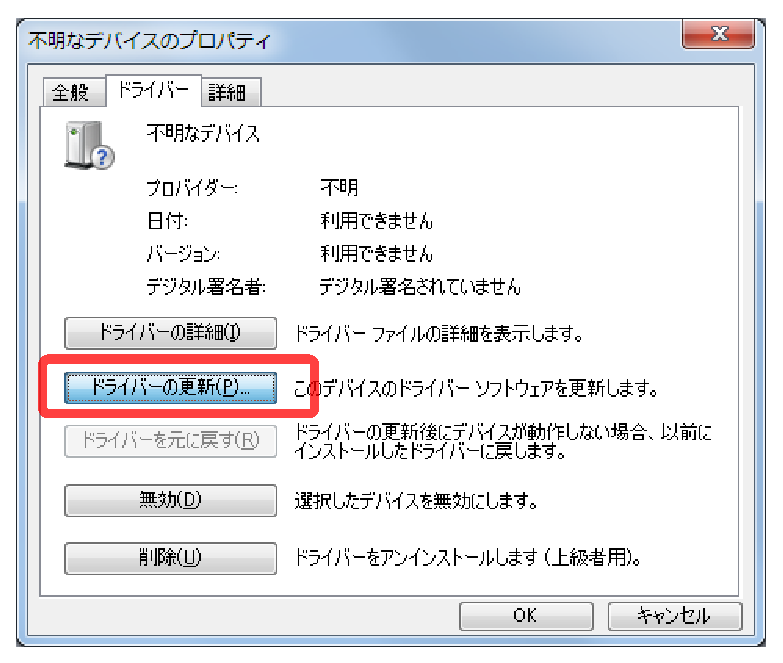
\includegraphics[width=72mm]{windriver-install.5.device_prop.eps}
			\caption{ドライバーの更新}
			\label{fig:windriver.device_prop}
		\end{figure}
	\item ``コンピュータを参照してドライバーソフトウェアを検索します(R)'' を選択
		\begin{figure}[H]
			\centering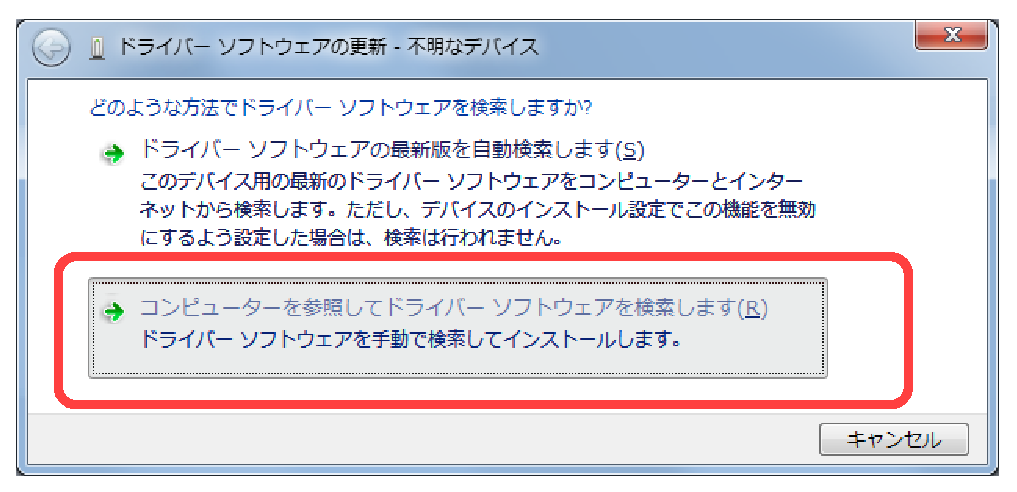
\includegraphics[width=94mm]{windriver-install.6.driversearch.eps}
			\caption{コンピュータを参照してドライバーソフトウェアを検索}
			\label{fig:windriver.driversearch}
		\end{figure}
	\item ``参照'' ボタンから、 ``SAM-BA for Windows'' をインストールしたディレクトリ下の ``drv'' ディレクトリを選択 (標準設定では C:{\textbackslash}Program~Files~(x86){\textbackslash}Atmel{\textbackslash}sam-ba\_2.12{\textbackslash}drv ) し、 ``次へ(N)'' を選択
		\begin{figure}[H]
			\centering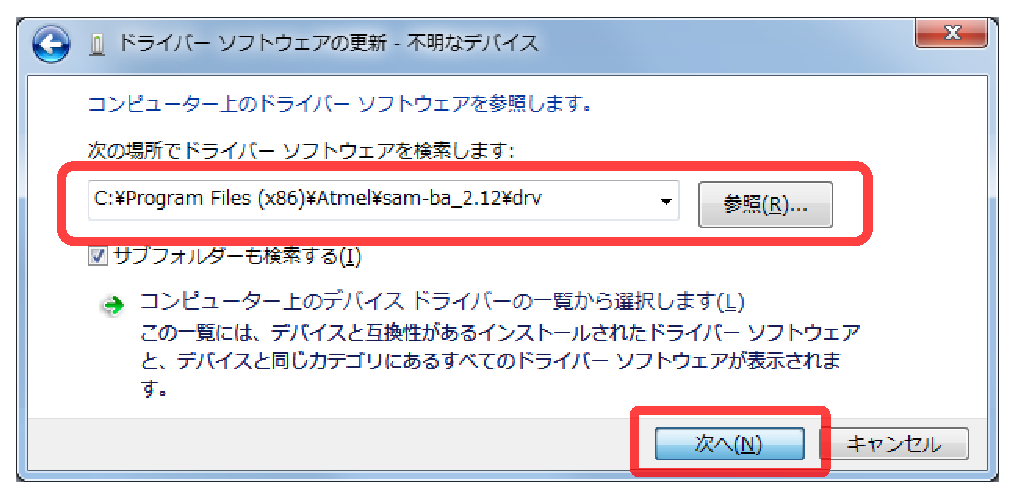
\includegraphics[width=94mm]{windriver-install.7.driverfile.eps}
			\caption{ドライバーソフトウェアを参照}
			\label{fig:windriver.driverfile}
		\end{figure}
	\item セキュリティ警告画面が現れるので、 ``このドライバーソフトウェアをインストールします(I)'' を選択
		\begin{figure}[H]
			\centering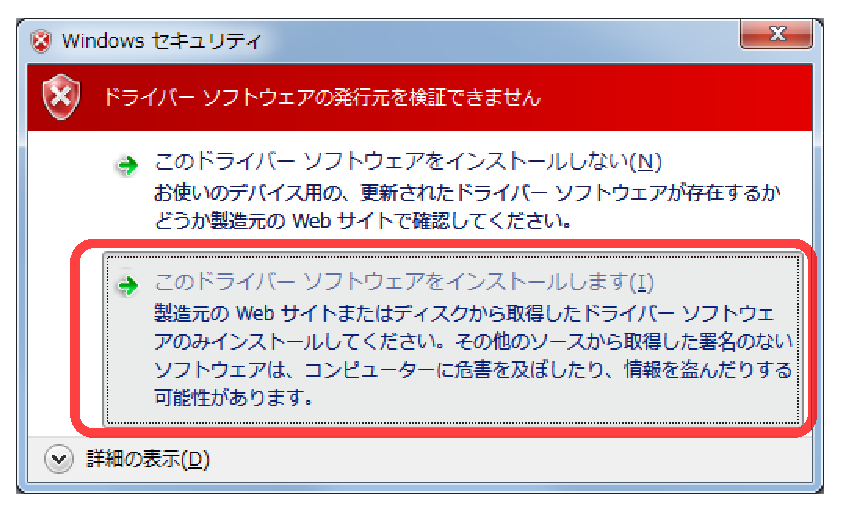
\includegraphics[width=76mm]{windriver-install.8.security.eps}
			\caption{ドライバーソフトウェアを参照}
			\label{fig:windriver.security}
		\end{figure}
\end{enumerate}
(Windows 8 以降では、署名無しのドライバインストールを許可する設定が必要です。)
\par

以下の手順に従ってファームウェアを書き込みます。
\begin{enumerate}
	\item インストールした ``SAM-BA for Windows'' を実行
	\item ``Select the connection'' 欄で、{\bf TF-2MD3-R6}のポートを選択
	\item ``Select your board'' 欄で、基板のバージョンに対応する型番を選択
		\begin{center}
		\begin{tabular}{rl}
			\hline
			{\bf プレ製品化版} & at91sam7se512-ek \\
			{\bf TF-2MD3-R6}   & at91sam7se256-ek \\
			\hline
		\end{tabular}
		\end{center}
	\item ``Connect'' を選択
		\begin{figure}[H]
			\centering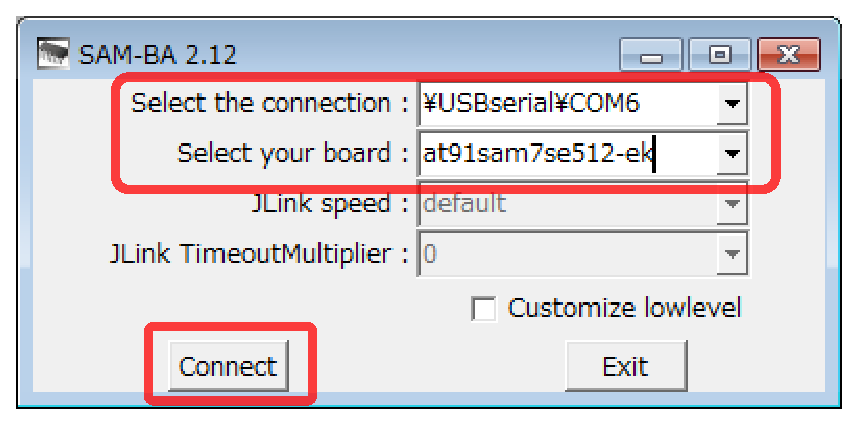
\includegraphics[width=80mm]{sam-ba.connect.eps}
			\caption{ ``SAM-BA for Windows'' 接続画面}
			\label{fig:sam-ba.connect}
		\end{figure}
	\item ``External RAM initialization failed.'' の警告が現れるので、 ``はい(Y)'' を選択
	\item ``Download / Upload File'' の ``Send File Name'' 欄で、コンパイル済みのファームウェアを開く
	\item ``Send File'' ボタンを選択
		\begin{figure}[H]
			\centering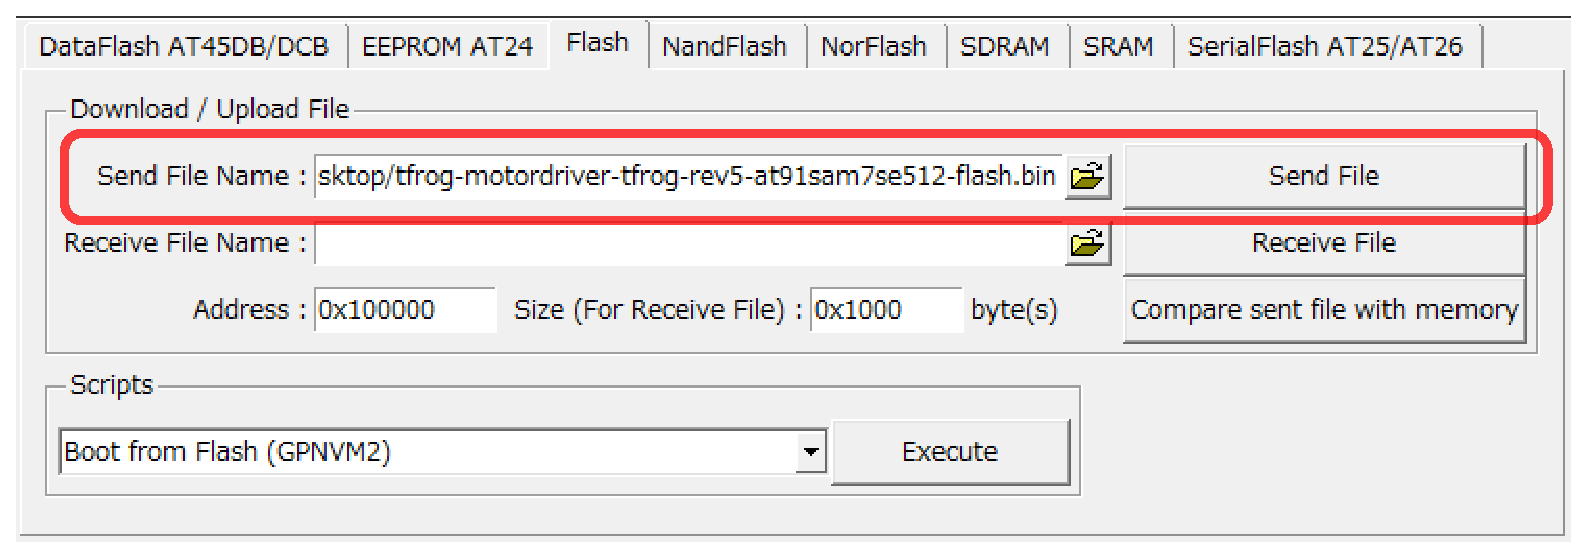
\includegraphics[width=148mm]{sam-ba.write.eps}
			\caption{ ``SAM-BA for Windows'' ファームウェア書き込み}
			\label{fig:sam-ba.write}
		\end{figure}
	\item ``Lock region(s)'' ウインドウが現れるので ``いいえ(N)'' を選択
	\item ``Scripts'' 欄で ``Boot from Flash (GPNVM2)'' を選択して ``Execute''
		\begin{figure}[H]
			\centering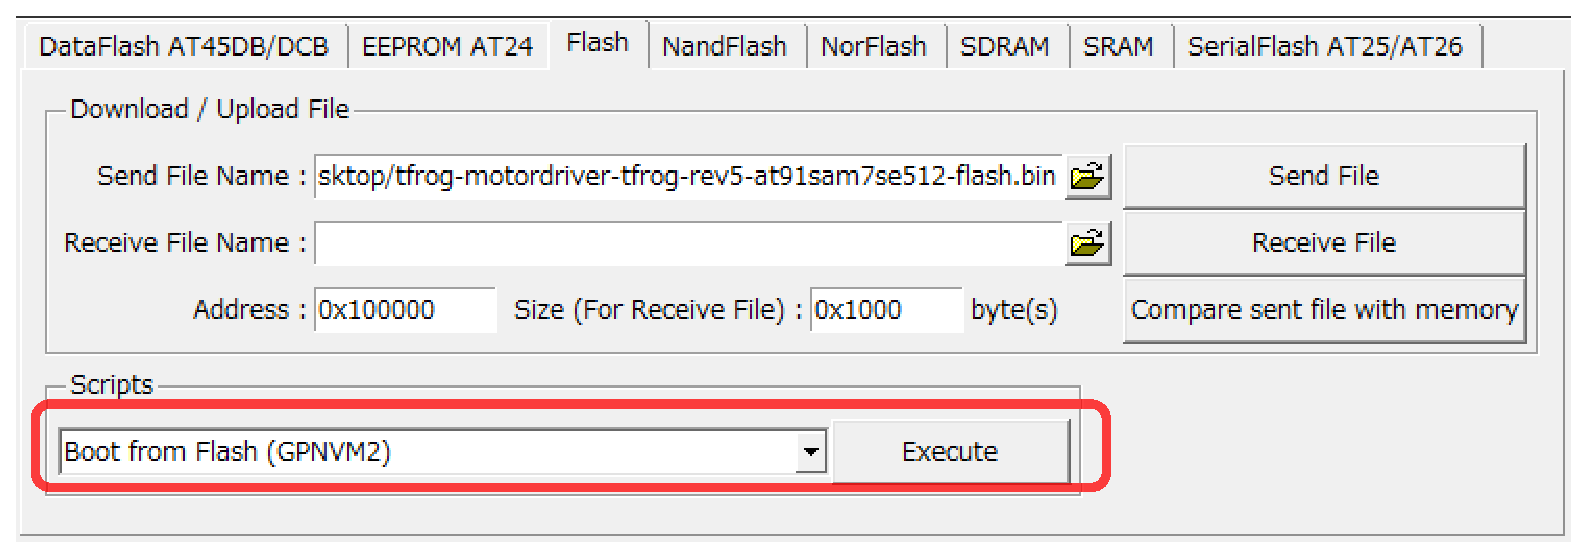
\includegraphics[width=148mm]{sam-ba.boot.eps}
			\caption{Flashからの起動設定}
			\label{fig:sam-ba.boot}
		\end{figure}
\end{enumerate}


作業が完了したら、コントローラ基板電源を切断し、再度、投入します。
\par

\bigskip
\warnbox{ファームウェア更新成功の確認}{
	\iconitem{warn.eps}{
		\item 電源投入時に、LED1が短時間点灯した後消灯、LED2が薄く点灯することを確認する
	}
}

% ---------------------------------------------------------------------
% --------------------------- subsection ------------------------------
\subsection{ファームウェアの書き込みに失敗する場合}
\label{sec:ハードウェア消去スイッチ}


上記の方法でファームウェアの書き込みに失敗する場合は、以下の手順で、FLASH ROM を強制的に消去することで書き込みが可能になる場合があります。

\begin{enumerate}
	\item {\bf TF-2MD3-R6}基板上のスライドスイッチ ``SW1'' を、1ピン表示側にスライド
	\item コントローラ基板電源(5V)を投入(1秒以内に消去が完了)
	\item コントローラ基板電源を切断
	\item スライドスイッチ ``SW1'' を、初期状態(3ピン表示側)にスライド
\end{enumerate}


なお、スライドスイッチ ``SW1'' は、基板の版ごとに以下の場所に実装されています。
\begin{description}
	\item [{\bf TF-2MD3-R6}] コントローラ基板の裏面中央 \\
		(ネジ止めされているドライブ基板とコントローラ基板を、取り外す必要があります。)
	\item [{\bf TF-2MD3 プレ製品化版}] コントローラ基板の表面中央
\end{description}


\newpage
% ******************************************************************
% **************************** section *****************************
\section{トラブルシューティング}
\label{sec:トラブルシューティング}

モータドライバが正しく動作しない場合の、問題の確認方法をご説明します。

% ---------------------------------------------------------------------
% --------------------------- subsection ------------------------------
\subsection{エラー表示LED}

モータドライバが動作を続けられない状態におちいった際、モータへの電力供給が停止され、基板上の{\bf LED1}が、エラー内容毎に、\tablename~\ref{tb:error_led}に示すパターンで点滅します。
各エラーは以下の状況で発生します。

\begin{description}
\itemsep=0.7em
\item [駆動電圧低下]\mbox{}\\
	モータ駆動用電源電圧が 8~V 以下になり回路が動作できなくなった場合に発生します。電源電圧が0.5秒間異常連続して復旧すると、自動的に動作を再開します。

\item [ホール素子1異常]\mbox{}\\
	ホール素子1の入力に、通常起こりえない信号パターンが与えられたときに発生します。例えば、ケーブルの配線が誤っている場合、断線、接触不良、短絡がある場合に発生します。

\item [ホール素子2異常]\mbox{}\\
	ホール素子1の場合と同様です。

\item [通信なし]\mbox{}\\
	速度制御などの指令値が、一定時間与えられなかった場合に発生します。コンピュータで動作している ypspur-coordinator が異常終了したり、CPU使用率が 100~\percent になり、通信ができない状態になっている可能性があります。

\end{description}

\newcommand{\ledon}{\hspace{-0.5em}\fcolorbox{black}{green}{\textcolor{green}{\small 点}}\hspace{-0.5em}}
\newcommand{\ledoff}{\hspace{-0.5em}\fcolorbox{black}{white}{\textcolor{white}{\small 消}}\hspace{-0.5em}}
\begin{table}[H]
\caption{エラー表示LED 点滅パターン}
\label{tb:error_led}
\smallskip
\centering\begin{tabular}{rcccccccccc}
\toprule
					& \multicolumn{10}{c}{1周期あたり 2.0秒  
						(点灯:\fcolorbox{black}{green}{\textcolor{green}{\small 点}}、
						 消灯:\fcolorbox{black}{white}{\textcolor{white}{\small 消}})} \\
\midrule\\[-5pt]
駆動電圧低下
		& \ledon & \ledon & \ledoff& \ledoff& \ledon & \ledon & \ledoff& \ledoff & \ledoff& \ledoff \\[12pt]
ホール素子1異常
		& \ledon & \ledoff& \ledon & \ledon & \ledon & \ledon & \ledon & \ledon  & \ledoff& \ledoff \\[12pt]
ホール素子2異常
		& \ledon & \ledoff& \ledon & \ledoff& \ledon & \ledon & \ledon & \ledon  & \ledoff& \ledoff \\[12pt]
通信なし
		& \ledon & \ledoff& \ledon & \ledoff& \ledon & \ledoff& \ledon & \ledoff & \ledoff& \ledoff \\[12pt]
\bottomrule
\end{tabular}
\end{table}
\newpage


% ---------------------------------------------------------------------
% --------------------------- subsection ------------------------------
\subsection{ypspur-coordinatorのエラー出力}

コンピュータで動作する ypspur-coordinator と、TF-2MD3 基板との通信中に発生する代表的なエラーの意味は以下の通りです。

\begin{description}
\itemsep=0.7em
\item [Error: Can't open serial port.]\mbox{}\\
	ypspur-coordinator が TF-2MD3 のUSBポートを開けない場合に発生します。TF-2MD3 のファームウェアが正しく書き込まれていない、もしくは ypspur-coordinator 起動時のポート指定が誤っている可能性があります。

\item [Error: Device doesn't have available YP protocol version.]\mbox{}\\
	通信開始時に TF-2MD3 が応答しない、もしくは異常な応答を返した場合に発生します。TF-2MD3 のファームウェアと ypspur-coordinator のバージョンに互換性がない、もしくはファームウェアが正しく書き込まれていない可能性があります。

\item [Error: Your parameter file format is too old.]\mbox{}\\
	TF-2MD3 のファームウェアが古い場合に発生します。

\item [Error: Your parameter file format is unsupported!]\mbox{}\\
	YP-Spur のバージョンが古い場合に発生します。

\item [Error: Cannot find parameter file.]\mbox{}\\
	ypspur-coordinator がロボットのパラメータファイルを読み込めない場合に発生します。ファイル名の指定が誤っている、もしくはパラメータファイルが読み込み禁止になっている可能性があります。

\item [Error: **** undifined!]\mbox{}\\
	ロボットのパラメータファイル中で、必須のパラメータ(****部分)が定義されていない場合に発生します。

\item [Error: Select in serial\_recieve failed. / Error: Read in serial\_recieve failed.]\mbox{}\\
	ypspur-coordinator が TF-2MD3 のUSBポートからデータを取得できない場合に発生します。TF-2MD3 の動作異常、もしくはUSBの通信が切断された可能性があります。

\item [Error: Select timed out. / Error: Read timed out.]\mbox{}\\
	ypspur-coordinator が TF-2MD3 のUSBポートからデータを取得できない場合に発生します。TF-2MD3 の動作異常、もしくはUSBの通信が切断された可能性があります。

\end{description}


\newpage
% ******************************************************************
% **************************** section *****************************
\section{問い合わせ先}
\label{sec:問い合わせ先}

\begin{itembox}[l]
	{ご購入方法、ハードウェアの不具合などについて}
	{
		\hspace{1em}{\bf ツジ電子株式会社}\par
		\medskip\hspace{2em}
		\parbox[H]{0.8\textwidth}{
			〒300-0013 茨城県土浦市神立町3739\\
			info2[at]tsuji-denshi.co.jp\\
			029-832-3031
		}
	}
\end{itembox}
\vspace{1em}
\begin{itembox}[l]
	{ソフトウェアのトラブルについて}
	{
		\hspace{1em}{\bf 渡辺敦志}\par
		\medskip\hspace{2em}
		\parbox[H]{0.8\textwidth}{
			〒305-8573 茨城県つくば市天王台1-1-1\\
			筑波大学 システム情報工学研究科 知能ロボット研究室(2013年度現在)\\
			atsushi.w[at]ieee.org\\
			029-853-5155
		}
	}
\end{itembox}
\vspace{1em}
\begin{itembox}[l]
	{技術的な質問、最新情報など}
	{
		\hspace{1em}{\bf T-frog プロジェクト モータドライバフォーラム (メーリングリスト)}\par
		\medskip\hspace{2em}
		\parbox[H]{0.8\textwidth}{
			\url{http://t-frog.com/forums/forum.php?ml=tf-2md3-devel}\\
			tf-2md3-devel[at]t-frog.com
		}
	}
\end{itembox}


\newpage
% ******************************************************************
% ************************ thebibliography *************************
\small
\begin{thebibliography}{99}
\thispagestyle{fancy}
\fancyhead[RO,RE]{参考文献}

\bibitem{the:dcm-ff-cur-cnt}
飯田重喜, 油田信一,
\newblock DCモータのソフトウェアサーボ系におけるフィードフォワード電流制御.
\newblock 電学論D Vol.109-D, No.4, pp.289-296, 1989.

\bibitem{the:pws_ff_cnt}
S. Iida, S. Yuta,
\newblock Control of Vehicle with Power Wheeled Steerings Using Feed-forward Dynamics Compensation, 
\newblock in Proc. of Annual Conference on the IEEE Industrial Electronics Society, pp. 2264-2269, 1991

\bibitem{the:vehicle_control}
坪内孝司,
\newblock 車輪移動体の制御, 
\newblock in Proc. of 日本ロボット学会主催 第43回講習会 ロボット工学入門シリーズ<移動技術編>『移動ロボットのやさしい解説』, pp. 58-68, 1995

\end{thebibliography}
\normalsize

\end{document}
